\section{Reelle (47ff) und komplexe Zahlen (53ff)}
Es wird erwartet, dass Sie die schon aus der Schule bekannten in den natürlichen, rationalen und reellen Zahlen gütigen Rechengesetze beherrschen: Dazu gehören die in Theorem 4.6 und Theorem 4.7 im Skript aufgelisteten Gesetze, insbesondere die Bruchrechnung, sowie die binomischen Formeln und die Potenzgesetze. Definition von Intervallen (alle Typen aus (4.11) sollten Sie kennen). Definition der komplexen Zahlen als Paare reeller Zahlen, Definition der komplexen Addition und Multiplikation. Definition von Realteil und Imaginärteil komplexer Zahlen. Definition von und Rechenregeln für komplexe/r Konjugation. Definition der Betragsfunktion reeller und komplexer Zahlen. Rechenregeln der Betragsfunktion, speziell Dreiecksungleichung und umgekehrte Dreiecksungleichung. Veranschaulichung der komplexen Zahlen und ihrer Arithmetik (speziell von Konjugation, Addition, Multiplikation und Betrag) in der komplexen Ebene. Regeln für endliche Summen und Produkte. 

\begin{figure}[H] \centering
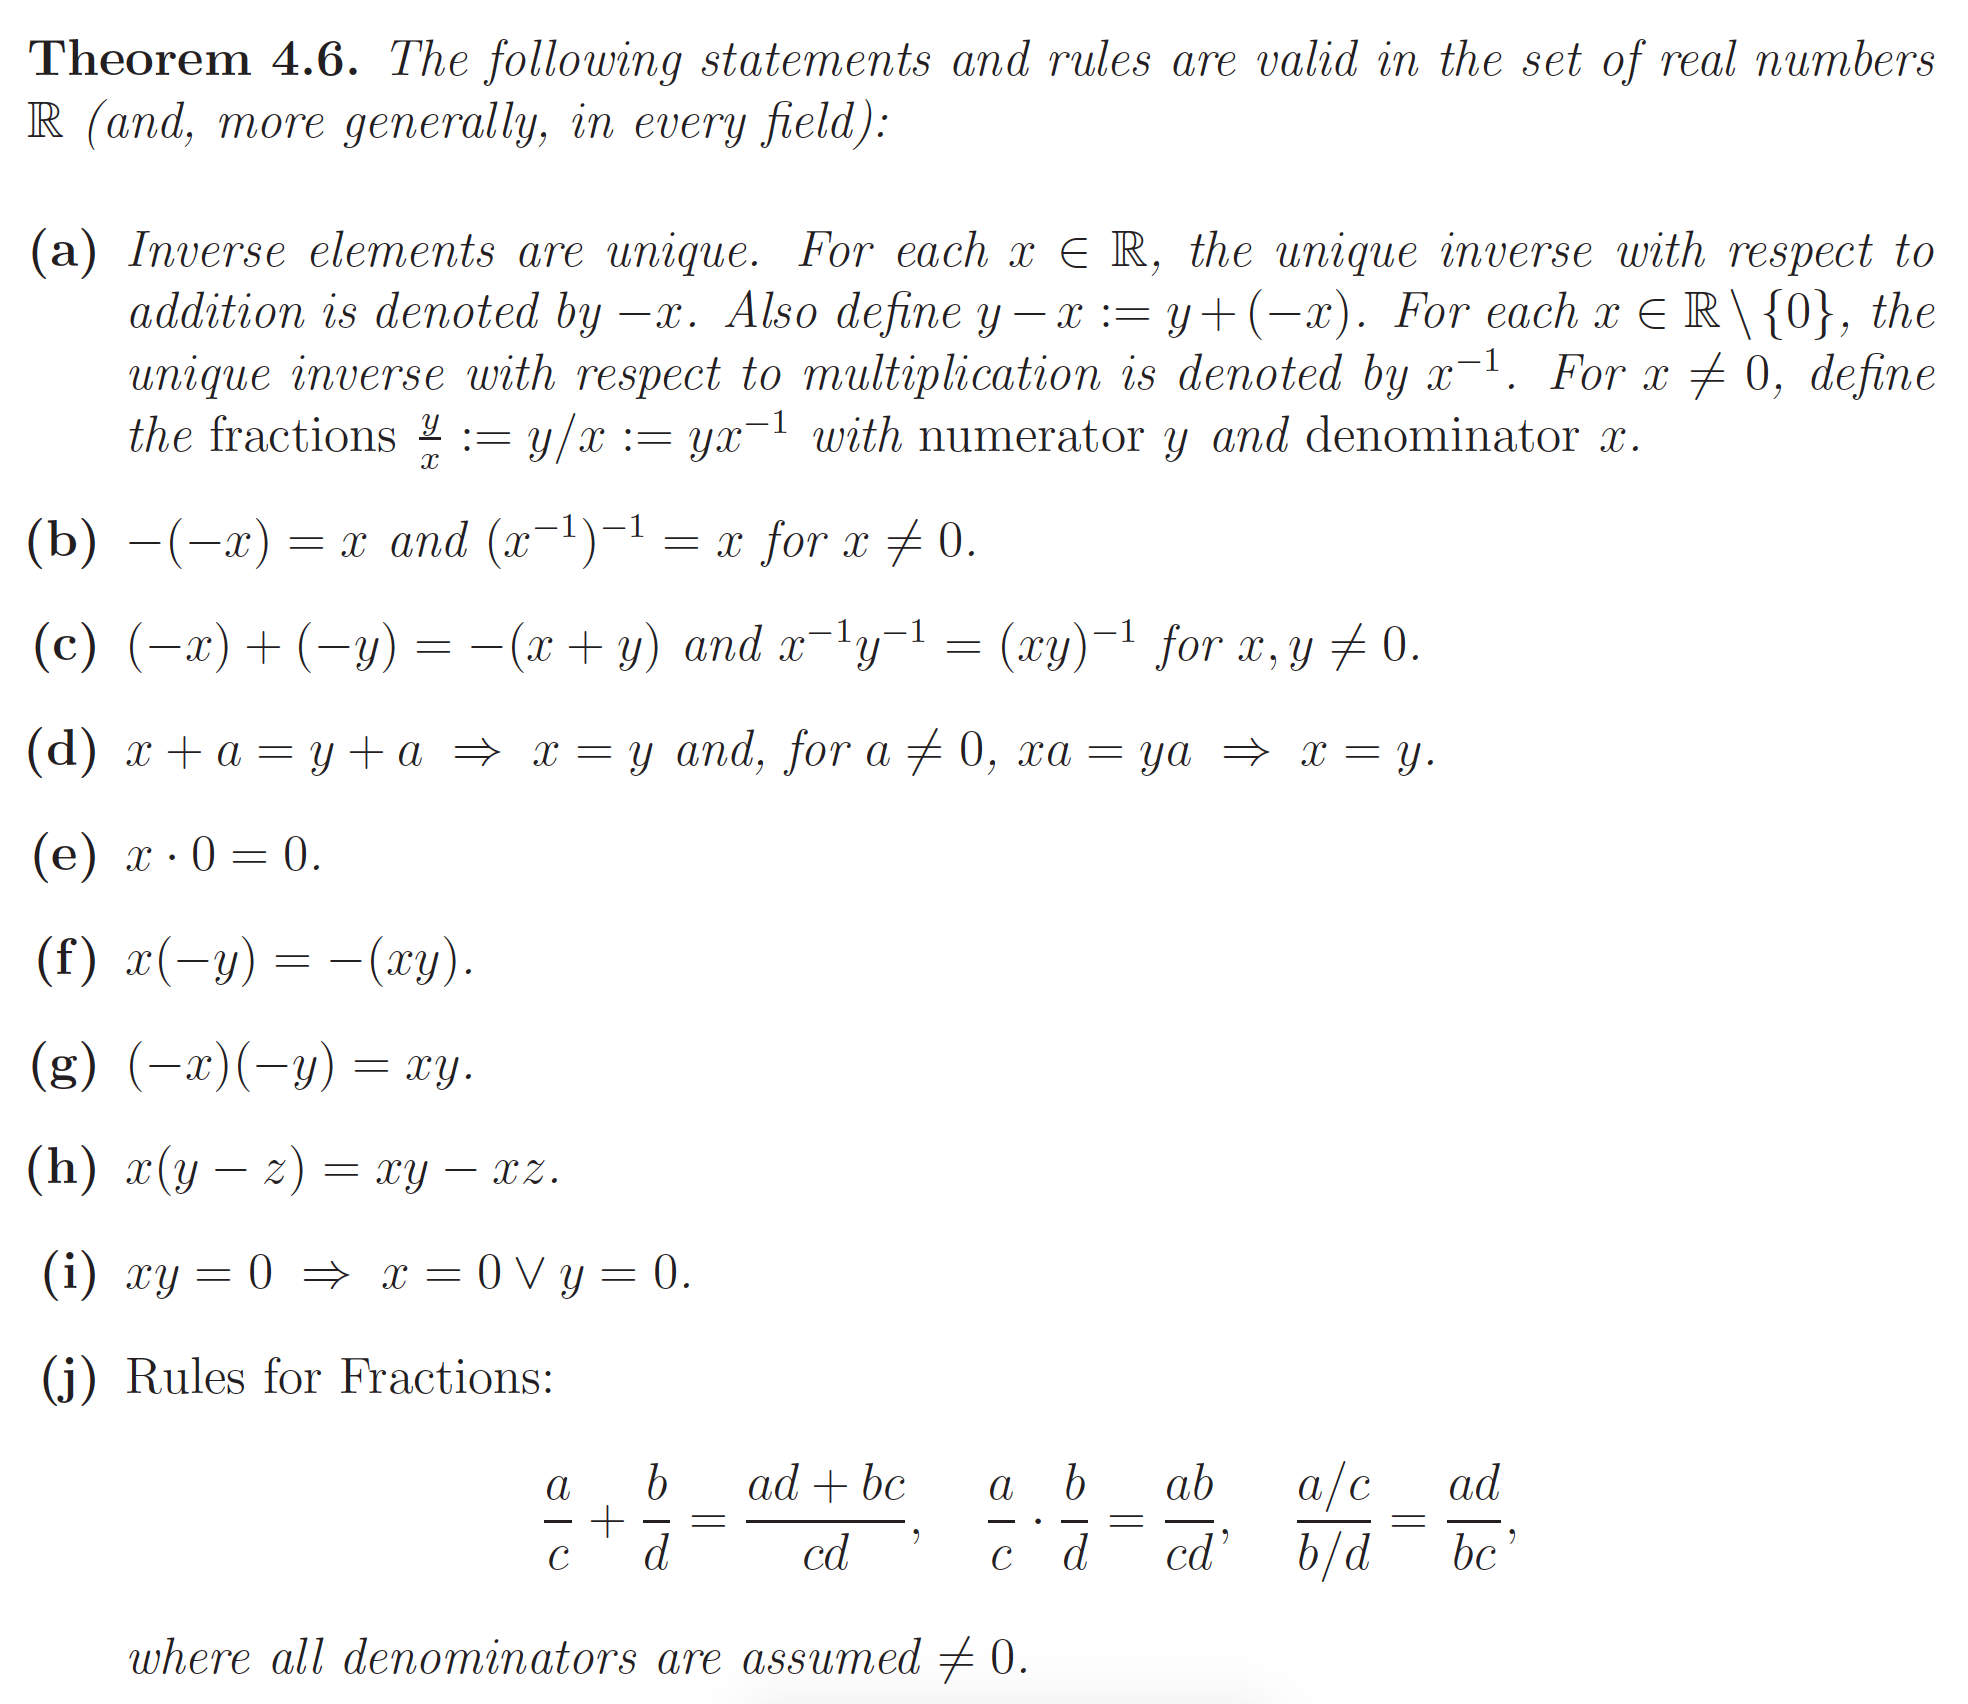
\includegraphics[width=0.7\textwidth]{media/4.png}
\end{figure}

\begin{figure}[H]
	\centering
  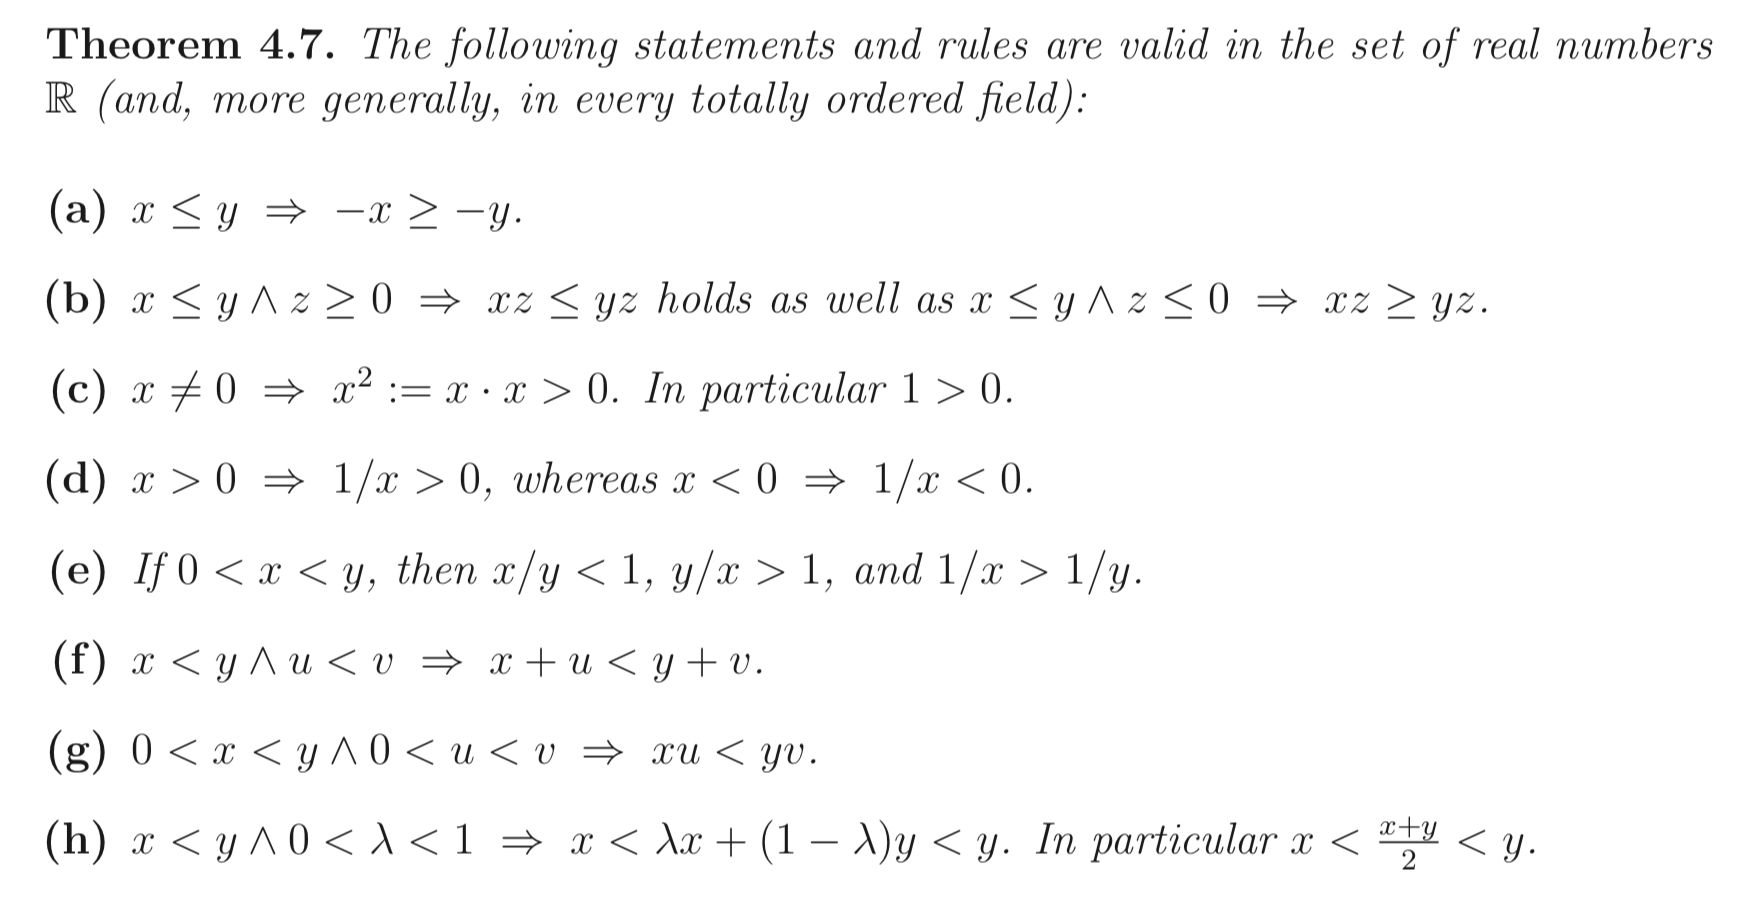
\includegraphics[width=0.7\textwidth]{media/50-theorem-4-7.png}
	\caption{50 theorem 4.7}
	\label{50_theorem_4.7}
\end{figure}

\subsection{Intervalle (alle Typen aus (4.11))}

\begin{figure}[H] \centering
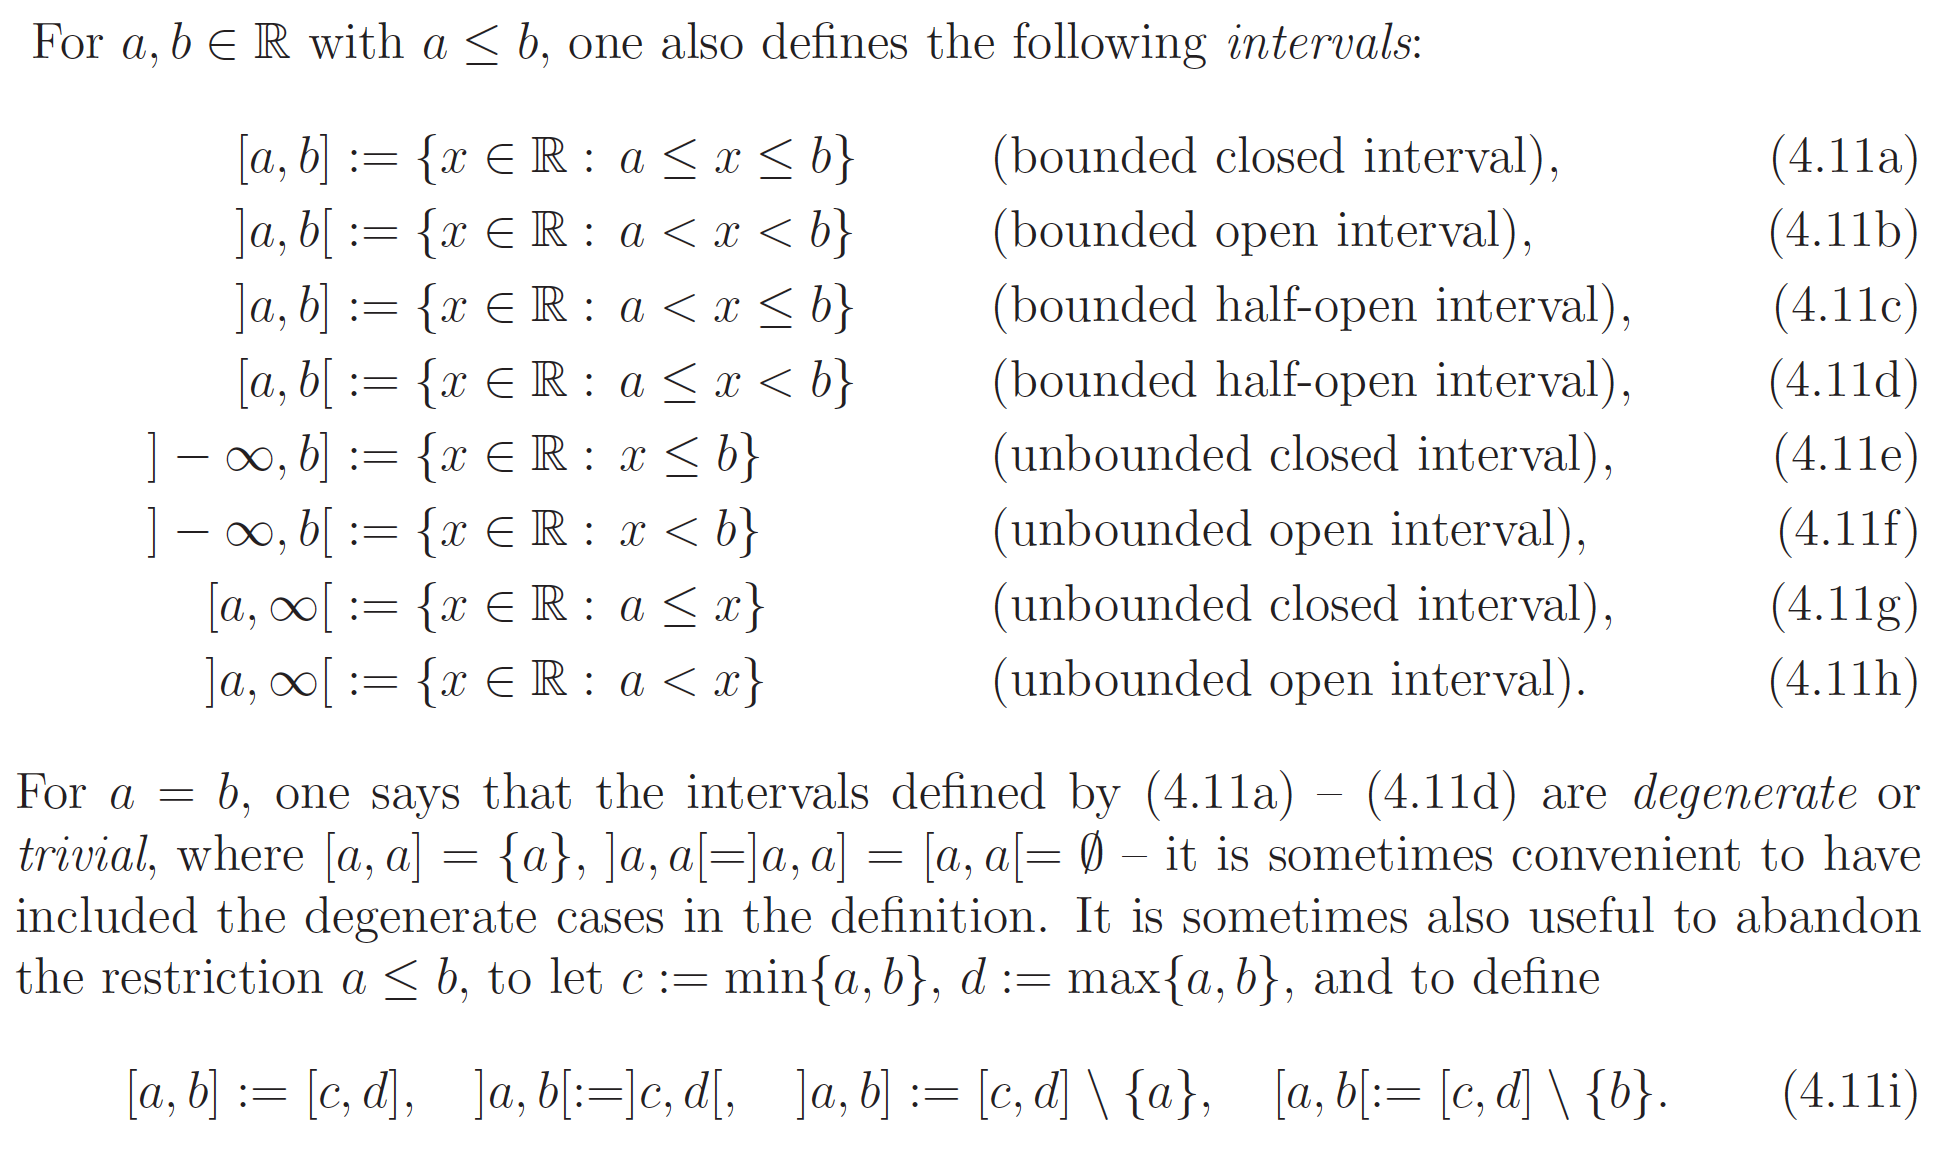
\includegraphics[width=0.7\textwidth]{media/4-1.png}
\end{figure}

\subsection{Definition der komplexen Zahlen als Paare reeller Zahlen (54), Definition der komplexen Addition und Multiplikation (53)}
$z \in \mathbb{C}:z=x+iy=(x,y), \quad \forall x,y \in \mathbb{R}$

$i^2=-1$

\begin{figure}[H]
	\centering
  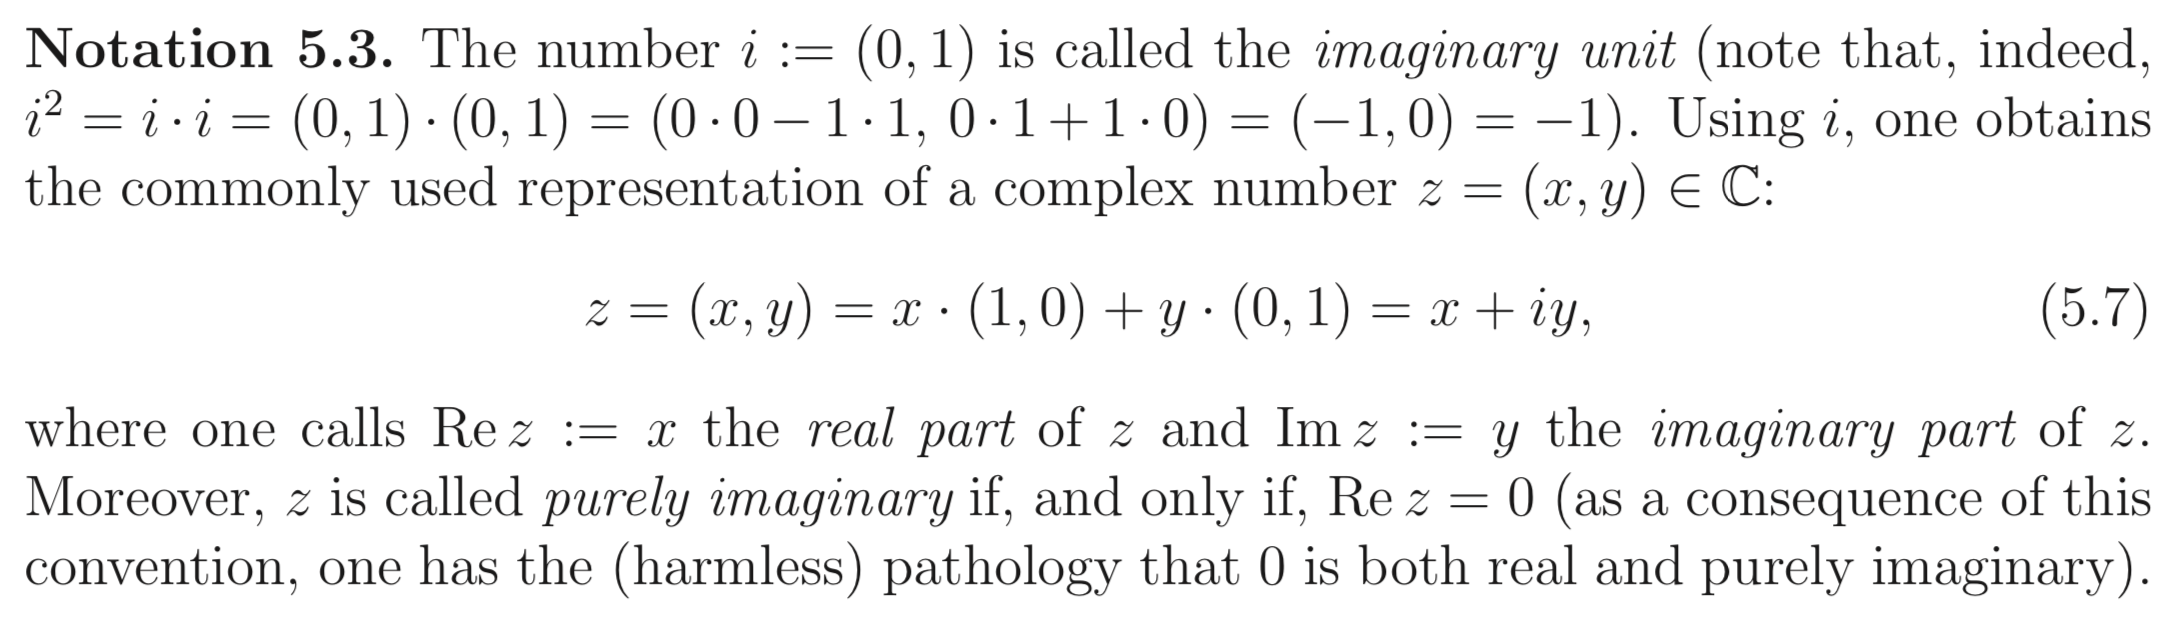
\includegraphics[width=0.7\textwidth]{media/54-notation-5-3.png}
	\caption{54 notation 5.3}
	\label{54_notation_5.3}
\end{figure}

\begin{figure}[H]
	\centering
  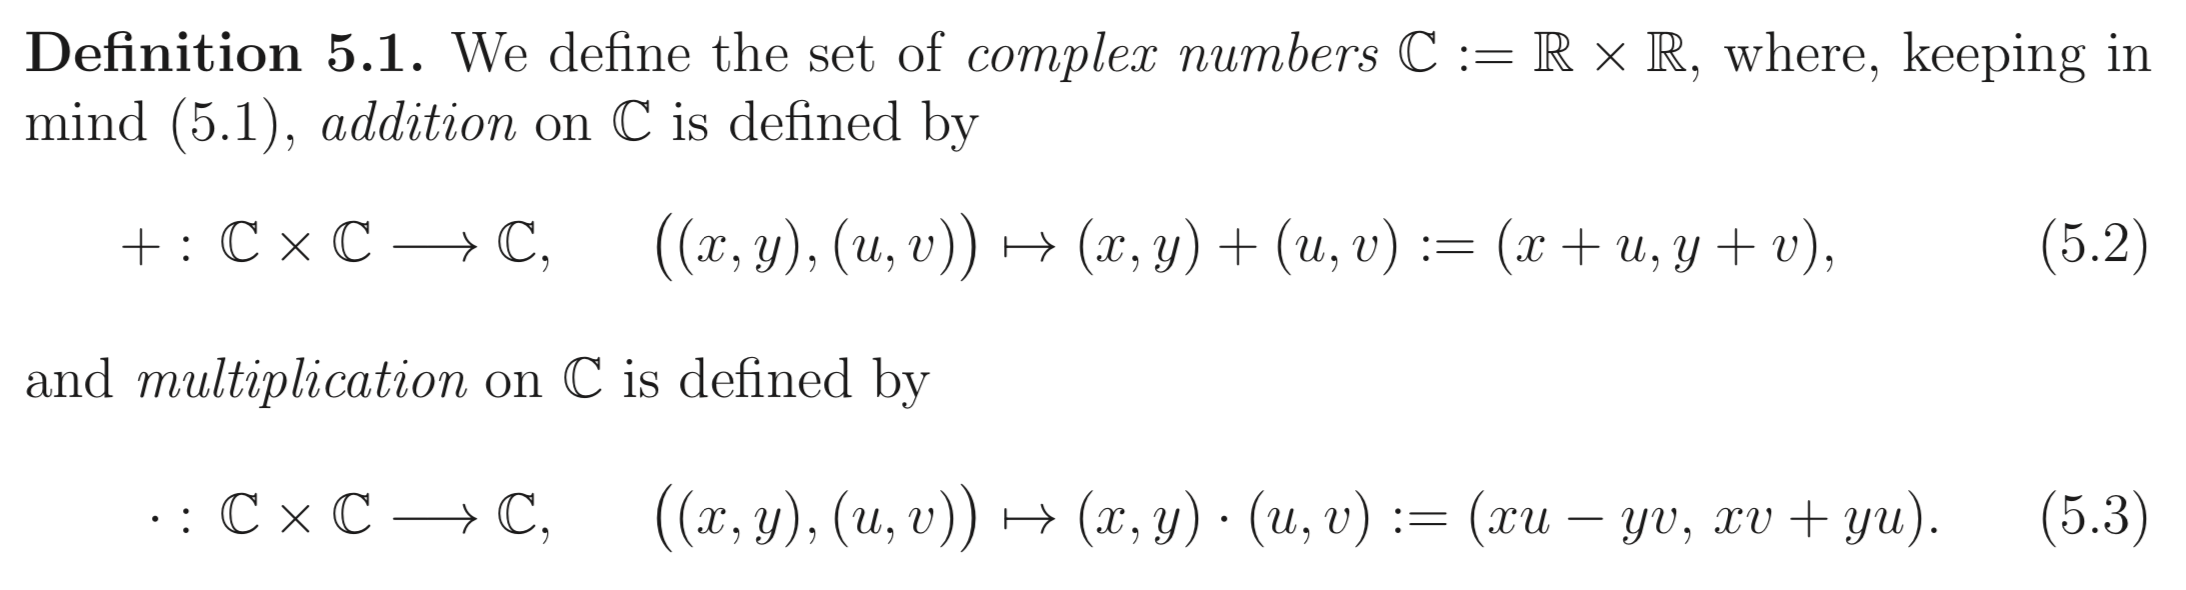
\includegraphics[width=0.7\textwidth]{media/53-definition-5-1.png}
	\caption{53 definition 5.1}
	\label{53_definition_5.1}
\end{figure}


\subsection{Definition von Realteil und Imaginärteil komplexer Zahlen (54)}
Komplexe Zahl $z = Re(z) + Im(z) = x + iy$

\subsection{Definition von und Rechenregeln für komplexe/r Konjugation (54f)}

\begin{figure}[H]
	\centering
  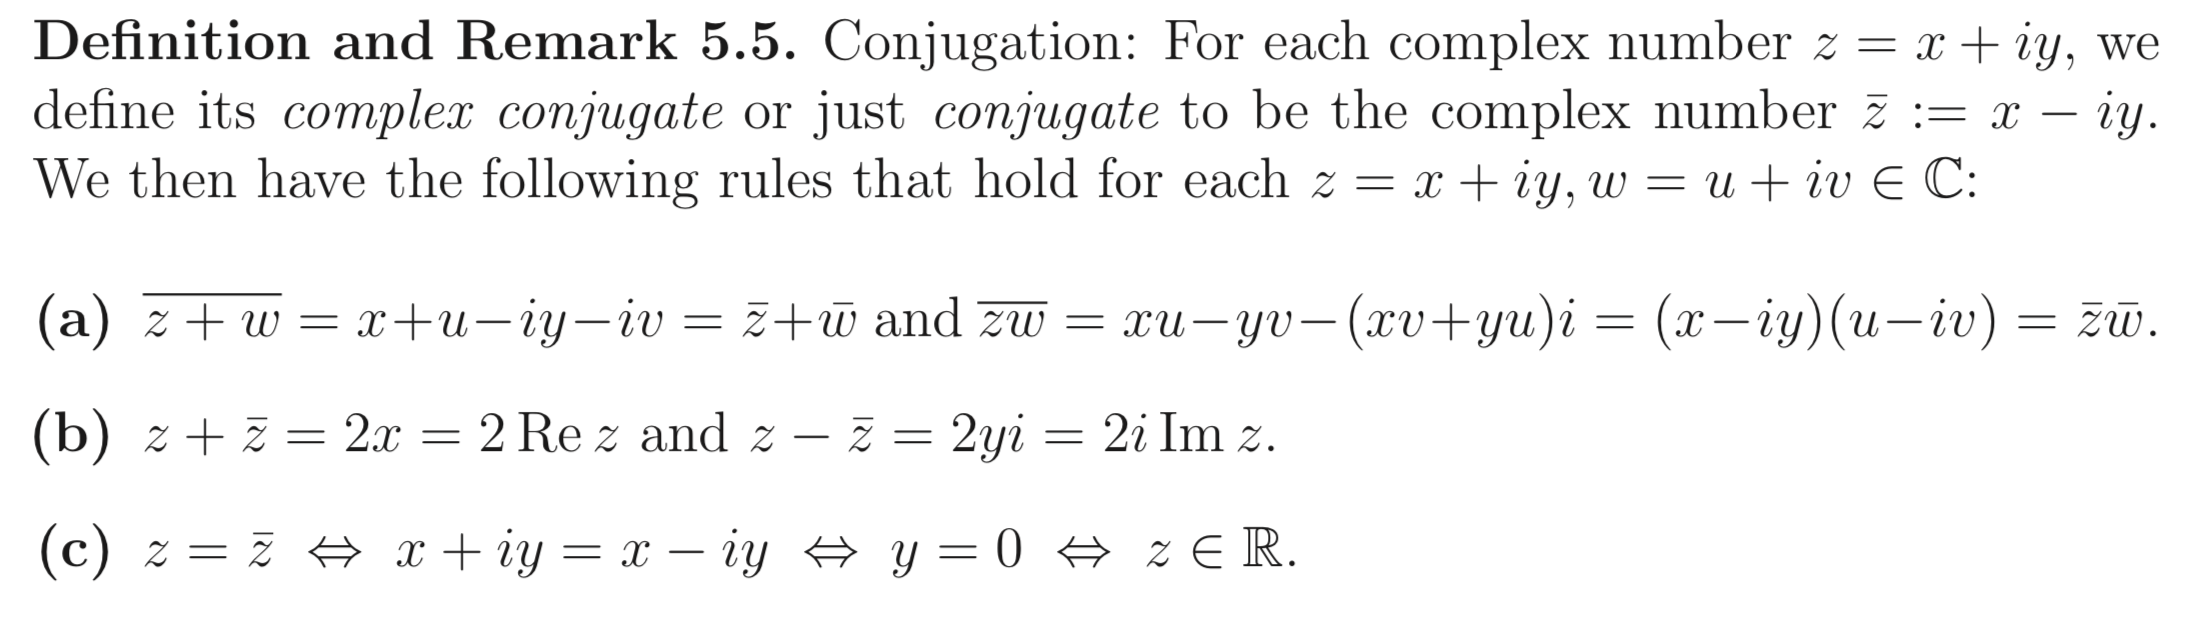
\includegraphics[width=0.7\textwidth]{media/54-defintion-5-5a.png}
	\caption{54 defintion 5.5a}
	\label{54_defintion_5.5a}
\end{figure}

\begin{figure}[H]
	\centering
  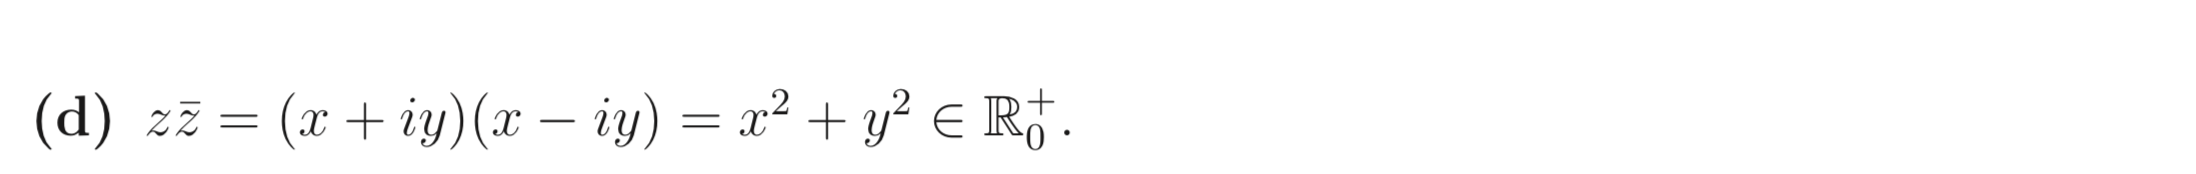
\includegraphics[width=0.7\textwidth]{media/54-defintion-5-5b.png}
	\caption{54 defintion 5.5b}
	\label{54_defintion_5.5b}
\end{figure}

\subsection{Definition der Betragsfunktion reeller und komplexer Zahlen (56)}

\begin{figure}[H]
	\centering
  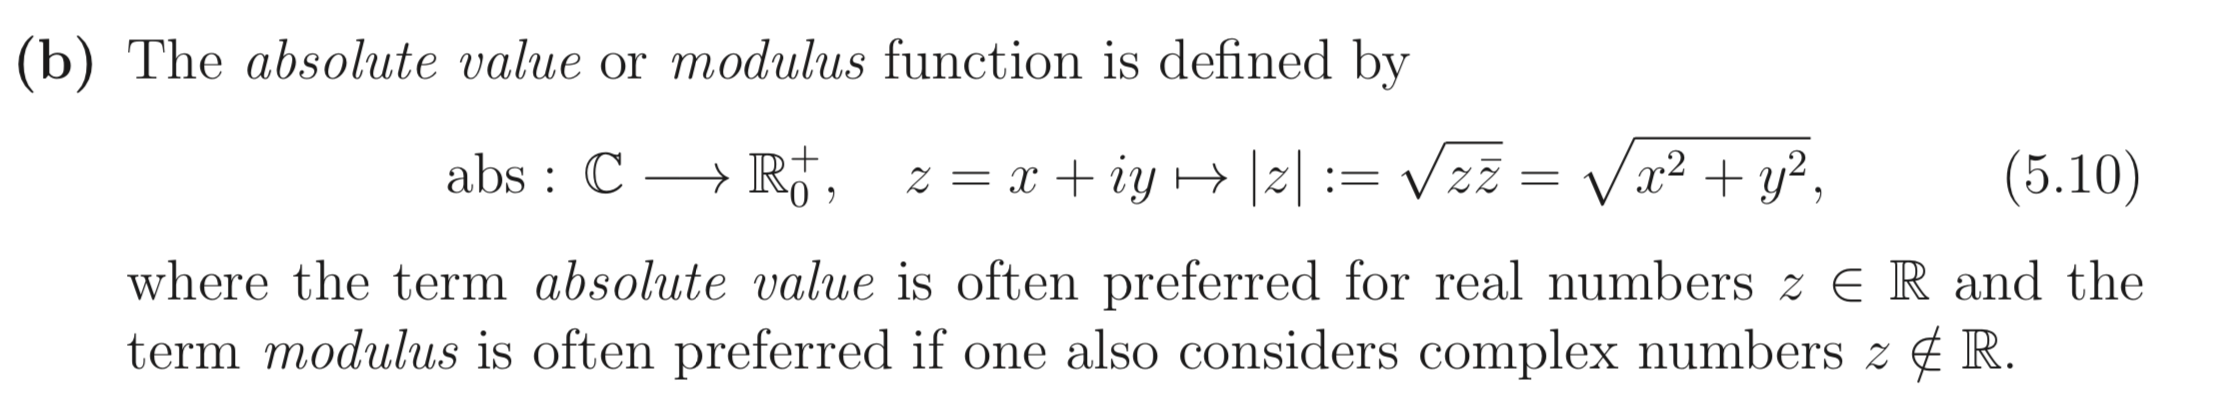
\includegraphics[width=0.7\textwidth]{media/56-defintion-5-9b.png}
	\caption{56 defintion 5.9b}
	\label{56_defintion_5.9b}
\end{figure}

\begin{figure}[H]
	\centering
  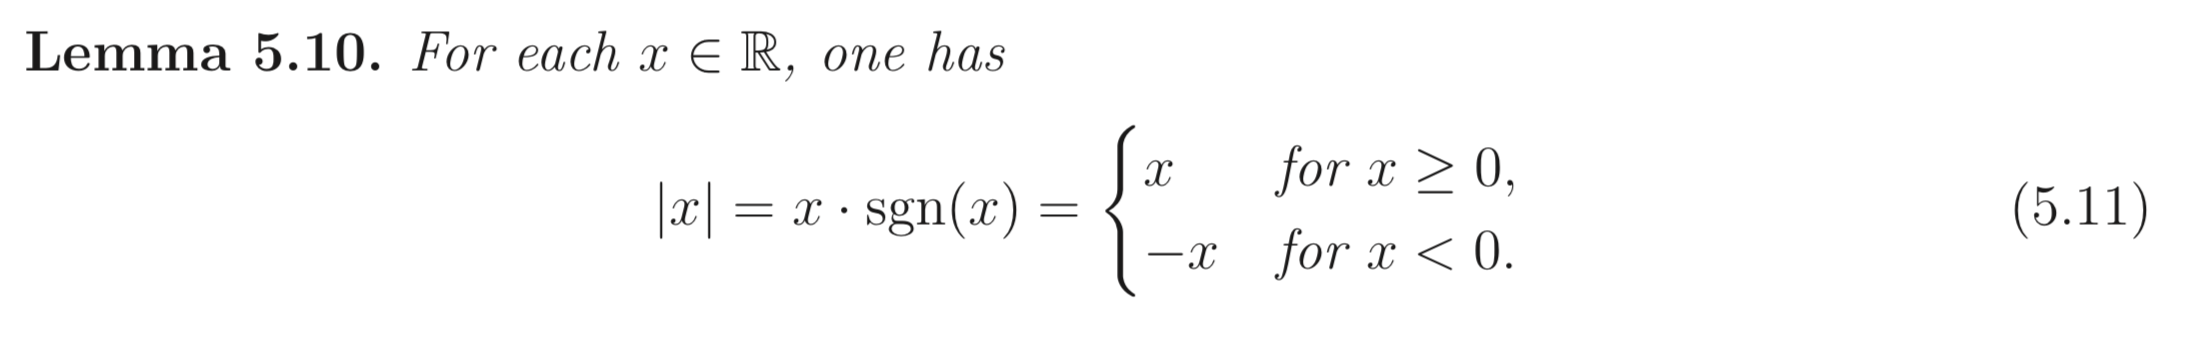
\includegraphics[width=0.7\textwidth]{media/56-lemma-5-10.png}
	\caption{56 lemma 5.10}
	\label{56_lemma_5.10}
\end{figure}

\subsection{Rechenregeln der Betragsfunktion, speziell Dreiecksungleichung und umgekehrte Dreiecksungleichung (57)}

\begin{figure}[H]
	\centering
  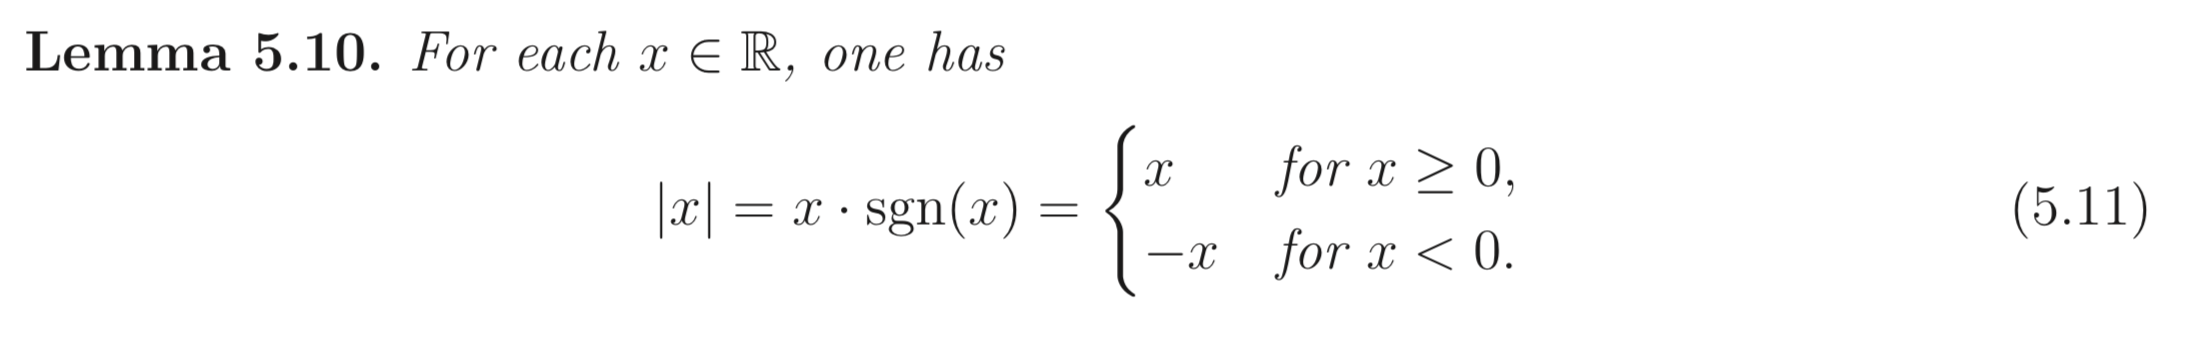
\includegraphics[width=0.7\textwidth]{media/56-lemma-5-10.png}
	\caption{56 lemma 5.10}
\end{figure}

\subsection{Veranschaulichung der komplexen Zahlen und ihrer Arithmetik (speziell von Konjugation, Addition, Multiplikation und Betrag) in der komplexen Ebene}
\TODO{???}

\subsection{Regeln für endliche Summen und Produkte (58f)}

\begin{figure}[H]
	\centering
  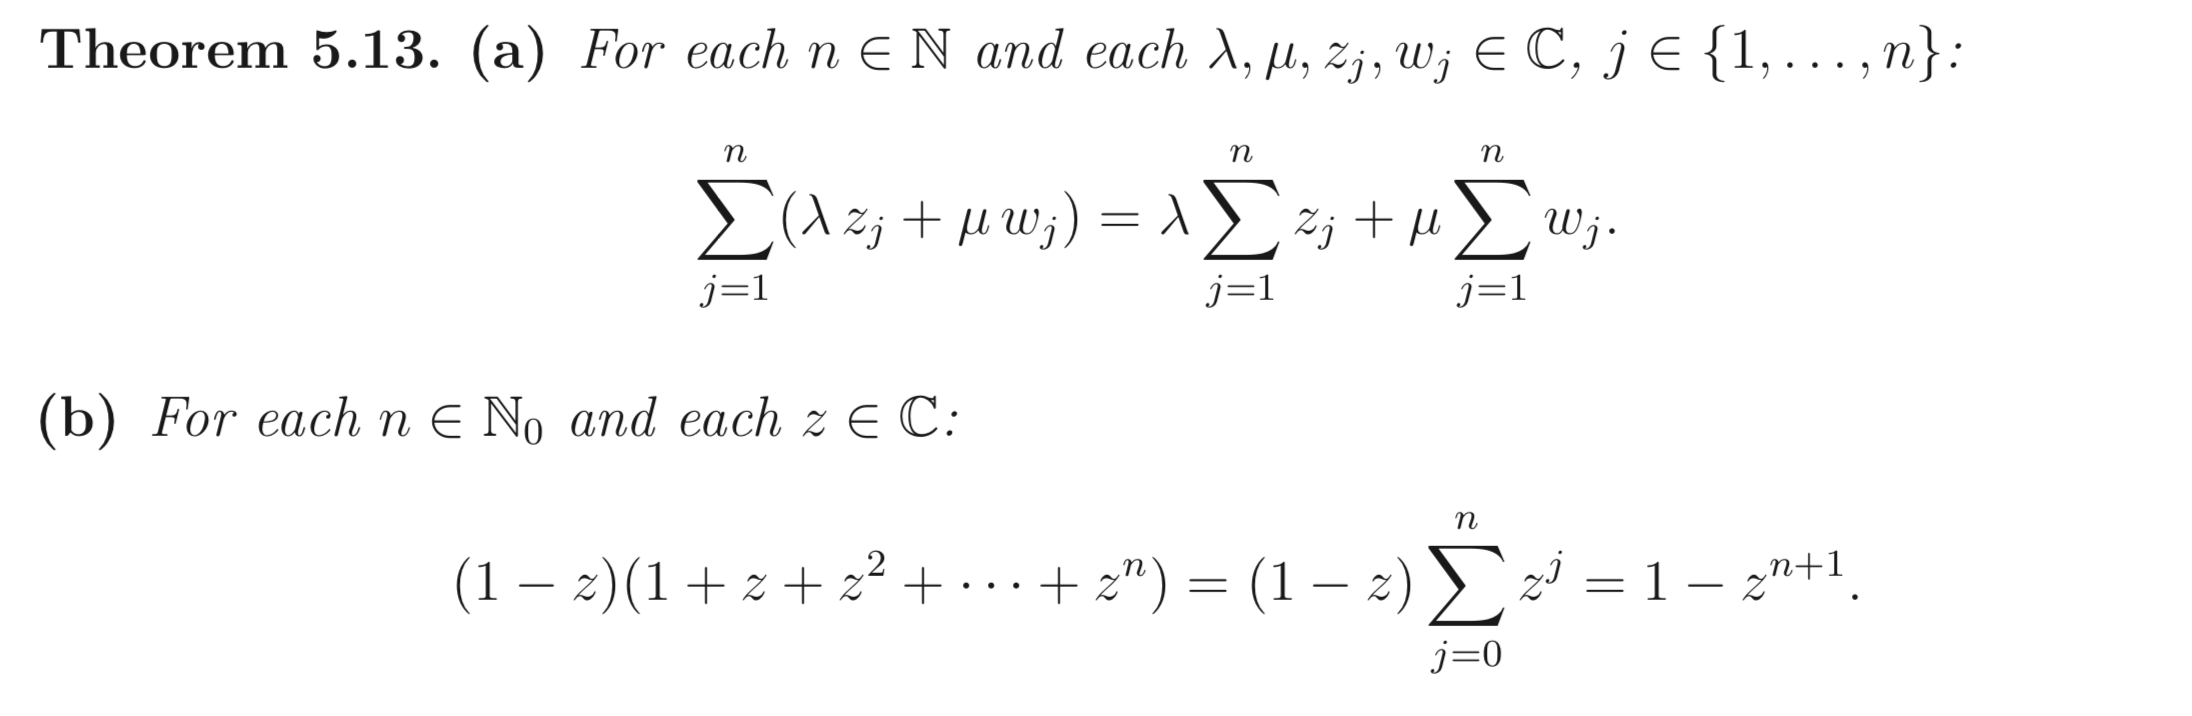
\includegraphics[width=0.7\textwidth]{media/58-theorem-5-13a.png}
	\caption{58 theorem 5.13a}
	\label{58_theorem_5.13a}
\end{figure}

\begin{figure}[H]
	\centering
  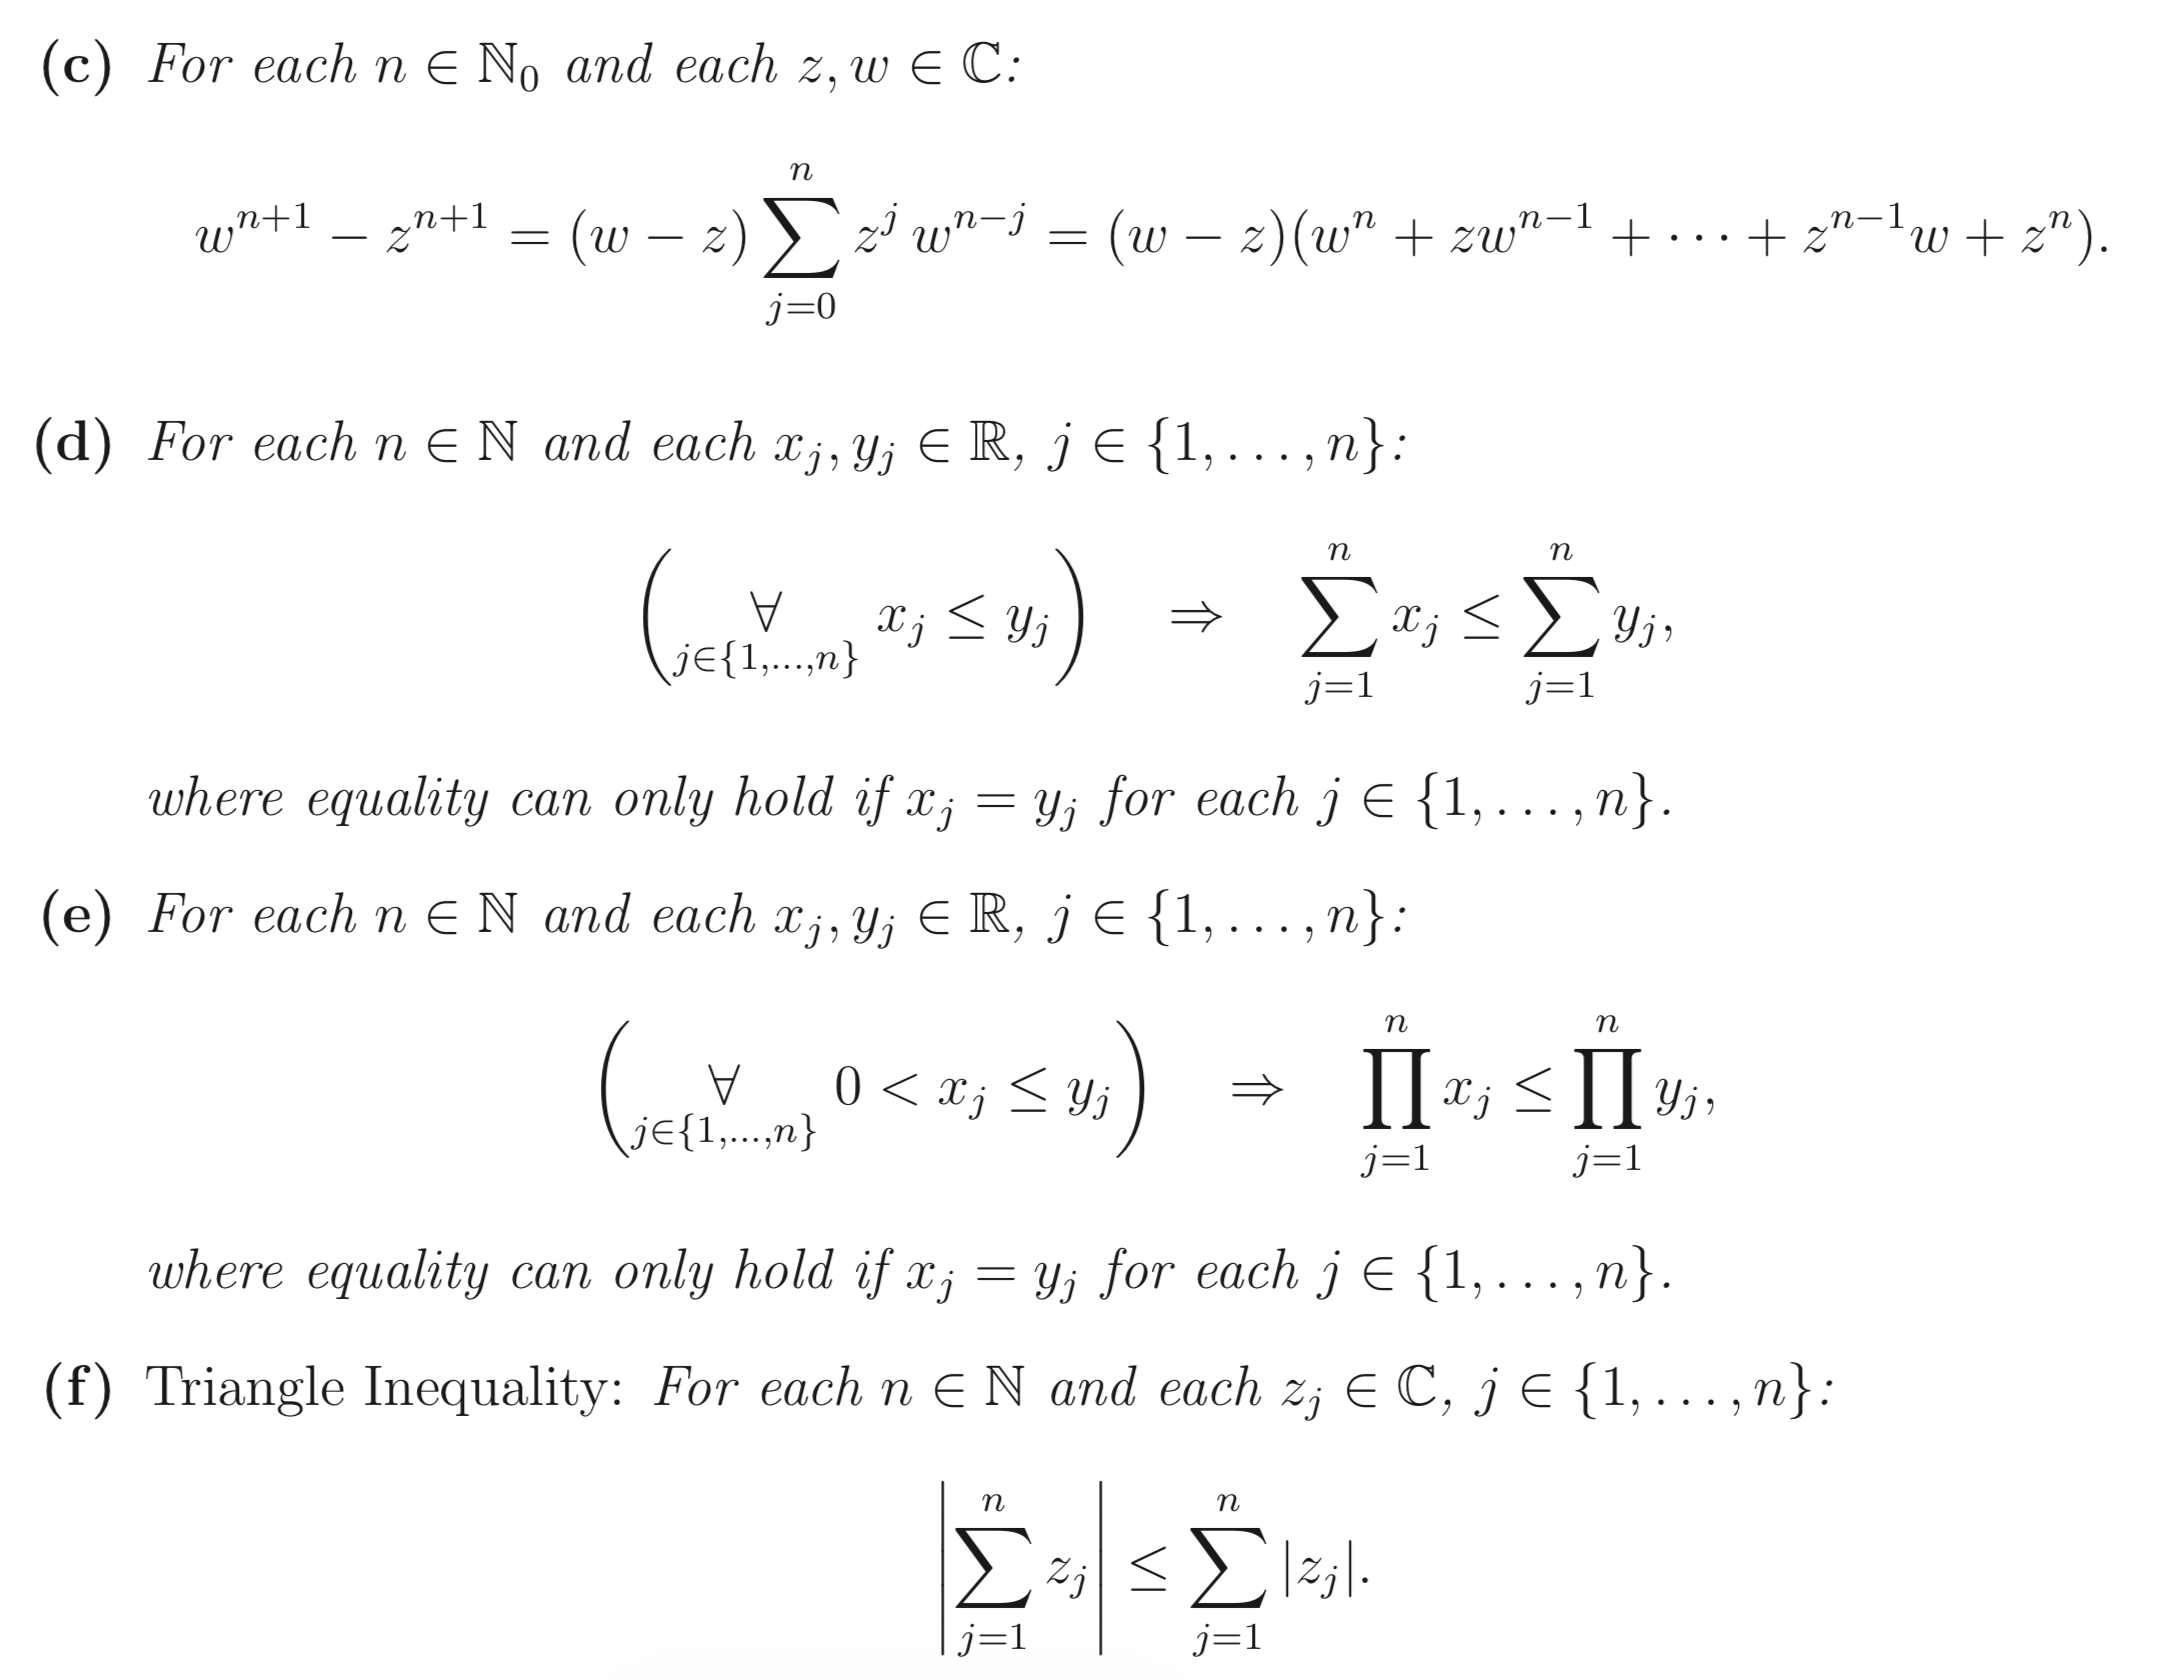
\includegraphics[width=0.7\textwidth]{media/58-theorem-5-13b.png}
	\caption{58 theorem 5.13b}
	\label{58_theorem_5.13b}
\end{figure}